\chapter{Methodology \& Implementation}

\renewcommand{\chaptername}{Chapter}
\section*{Introduction}

This chapter details the methodology and implementation of the proposed path planning system for logistics forklifts, 
focusing on guiding the robot to a pallet in the tight spaces of a warehouse. The system uses pattern-based paths with 
splines, optimized by meta-heuristic algorithms, to navigate efficiently in these confined areas. The chapter begins with 
an overview of the design structure, followed by a clear explanation of the steps and techniques used to ensure 
smooth and accurate movement toward the pallet. Implementation details are then covered, showing how the system 
components are integrated into a cohesive solution for precise pallet access within the warehouse environment.

\section{Methodology }
%goals and overall approach of the methodology
Considered the problems detailed in chapter 1, the following goals were identified based on the company's vision and the 
general requirements for applications to autonomous mobile robots in intralogistics:
\begin{itemize}
    \item Explainability and robustness of mobile robot behavior
    \item Accuracy of the solution and station relation
    \item Optimization of paths:
    \item Obstacle avoidance
\end{itemize}

Starting with the operating environment, the stations, the focus was on the problems inside. The issue of linking 
the forklifts in the near-field to the pallet is nothing but new to the intralogistics sector. 
The process is repeated dozens of times daily inside warehouses and factories where forklift drivers take control over 
resolving the problem. Taking a deeper look at their approaches to resolve the same issue, the autonomous vehicles team 
noticed that forklift drivers have certain driving styles that are repeated according to the current situation.
Just like car parking, depending on the type of the parking slot, there are some patterns to reproduce in order to fit 
the car inside its assigned spot as given by figure \ref{Parking Styles}. Assisted car parking support is 
embedded in human-driven and driverless cars to instill safety and order.

\begin{figure}
    [H]
    \begin{center}
    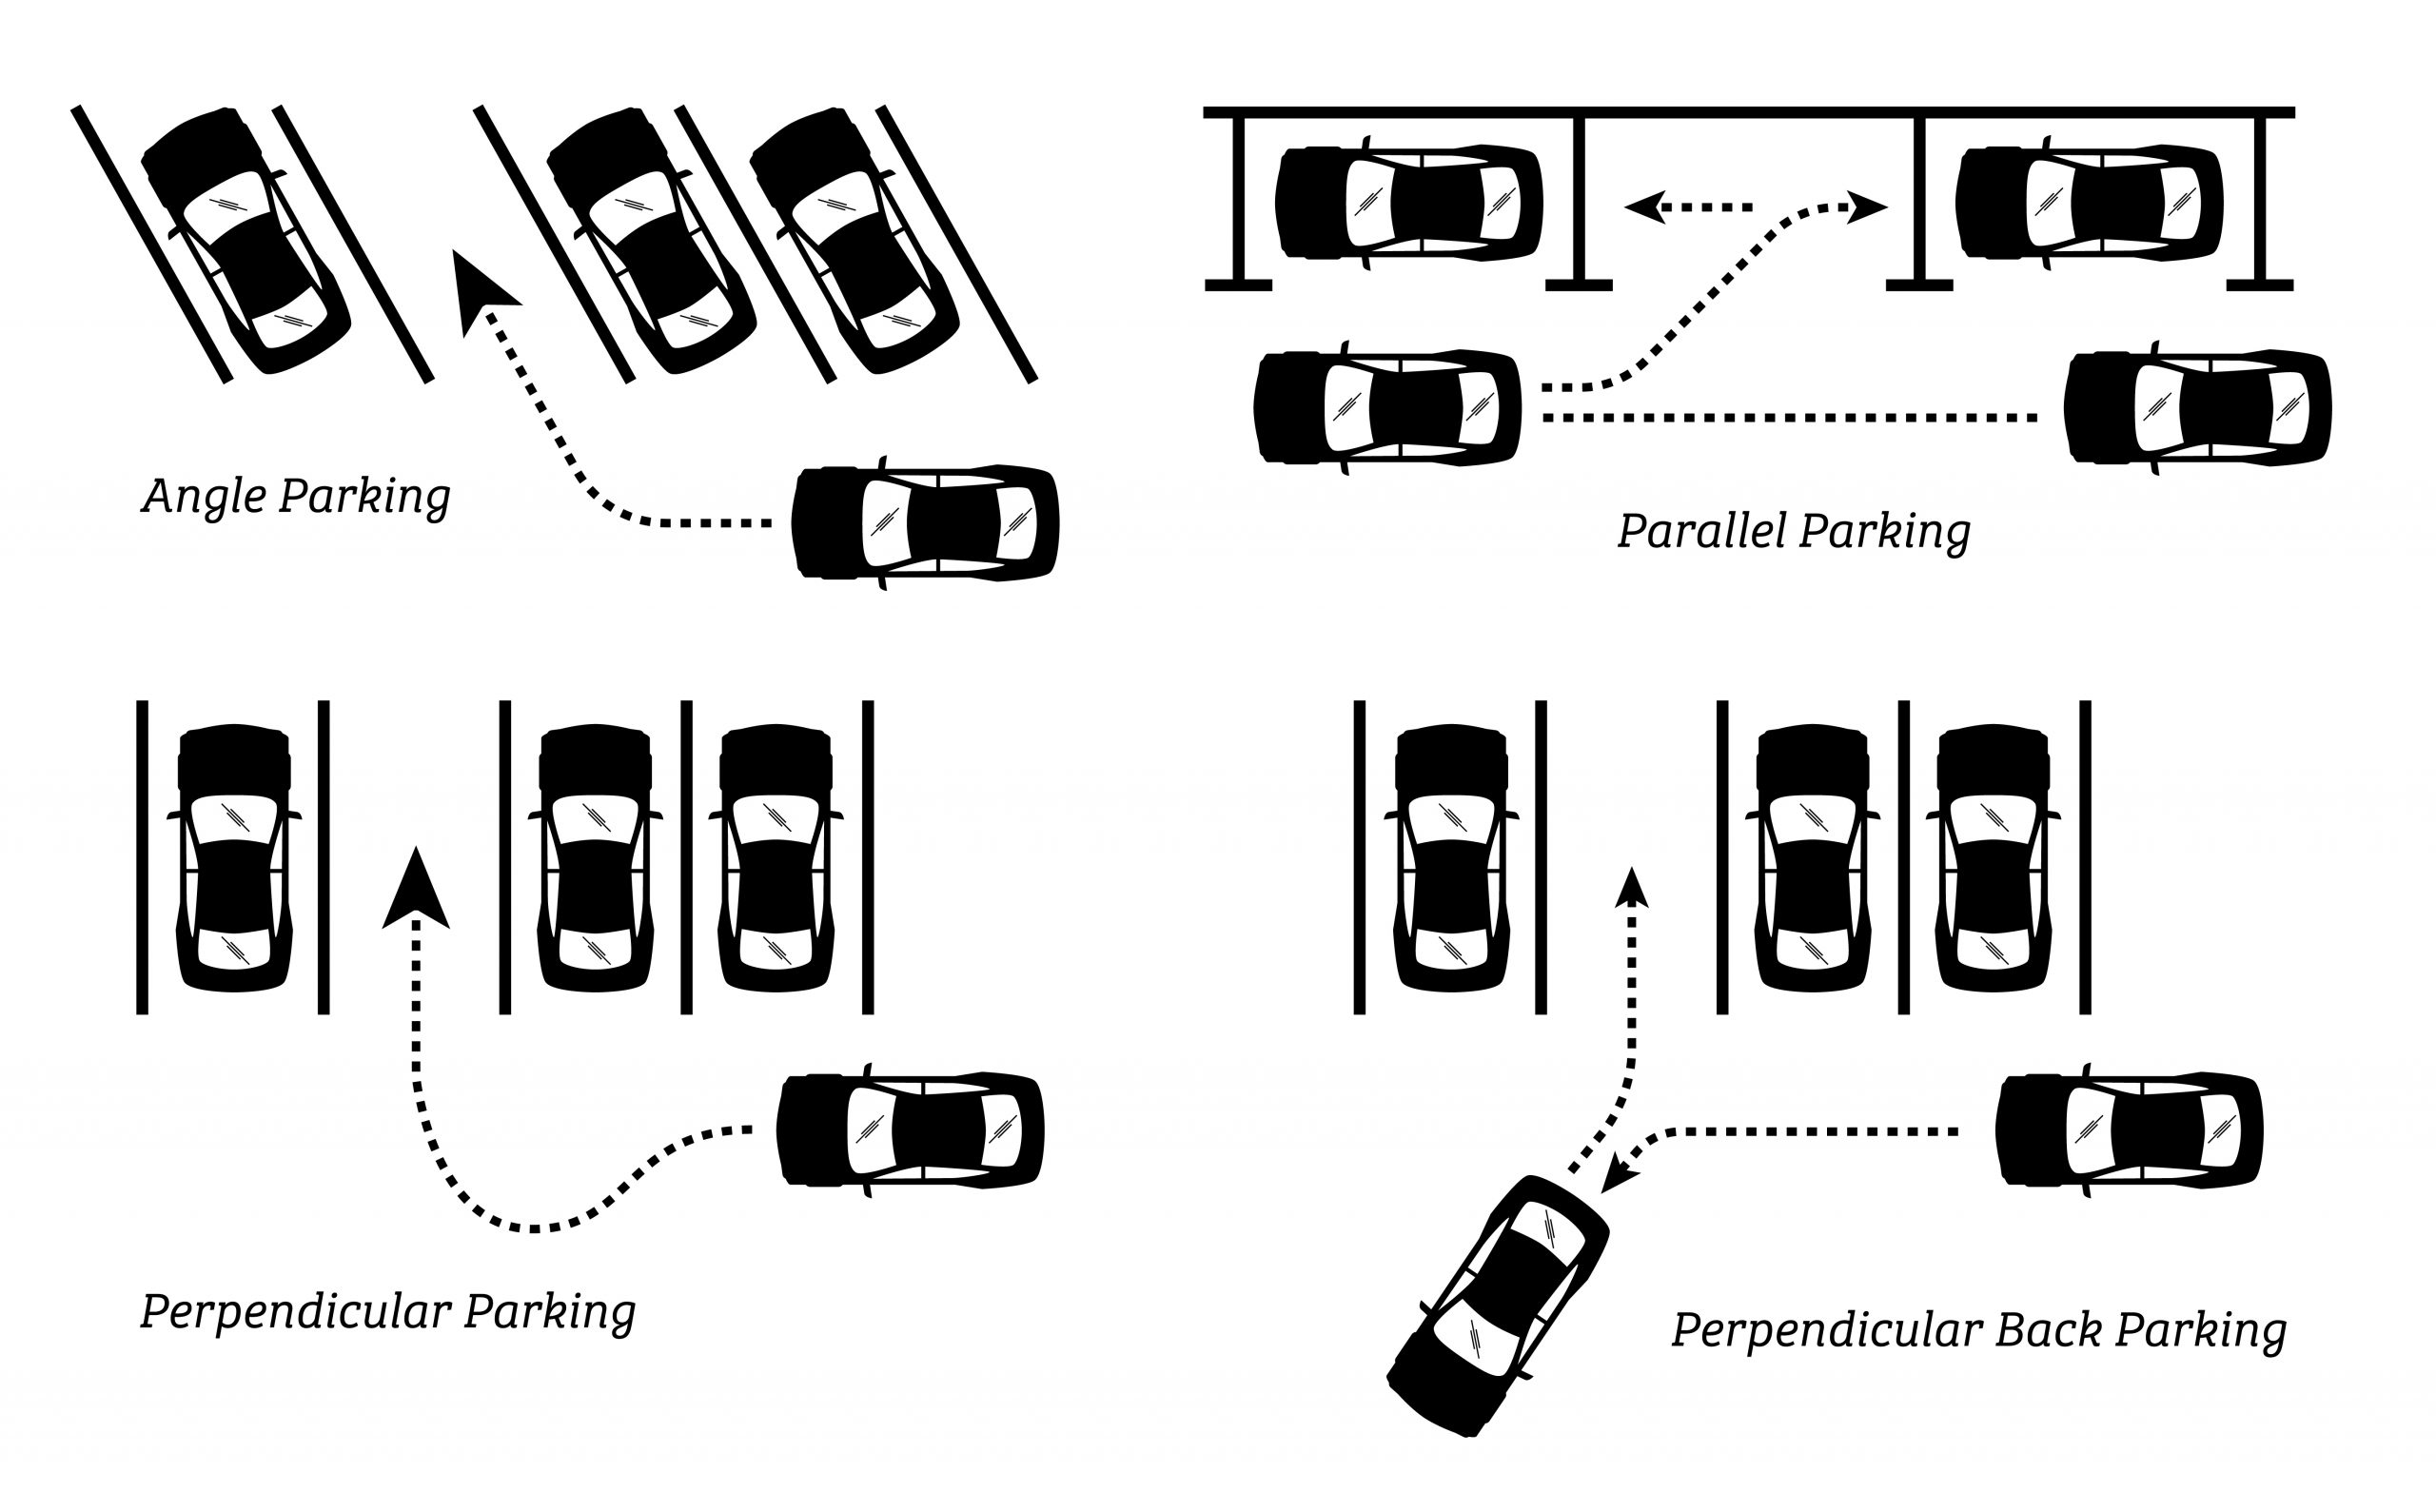
\includegraphics[width=4in]{images/Chap2/perpendicular-parking-a-lot-scaled.jpg}\\
    \caption{Parking Styles}
    \label{Parking Styles}
    \end{center}
\end{figure}

After the truck arrives in the station, the drivers would drive and steer in opposite direction of the pallet, until the 
forks are in a position to easily and correctfully drive to the pallet in fork direction.
The goal here is to develop a pallet-linking assistance algorithm to facilitate the driving and pallet pickup process for 
autonomous forklifts as given by figure \ref{pattern}. The truck would autonomously plan the path to its destination
based on the pattern and on the environment settings that he will navigate in. 

\begin{figure}
    [H]
    \begin{center}
    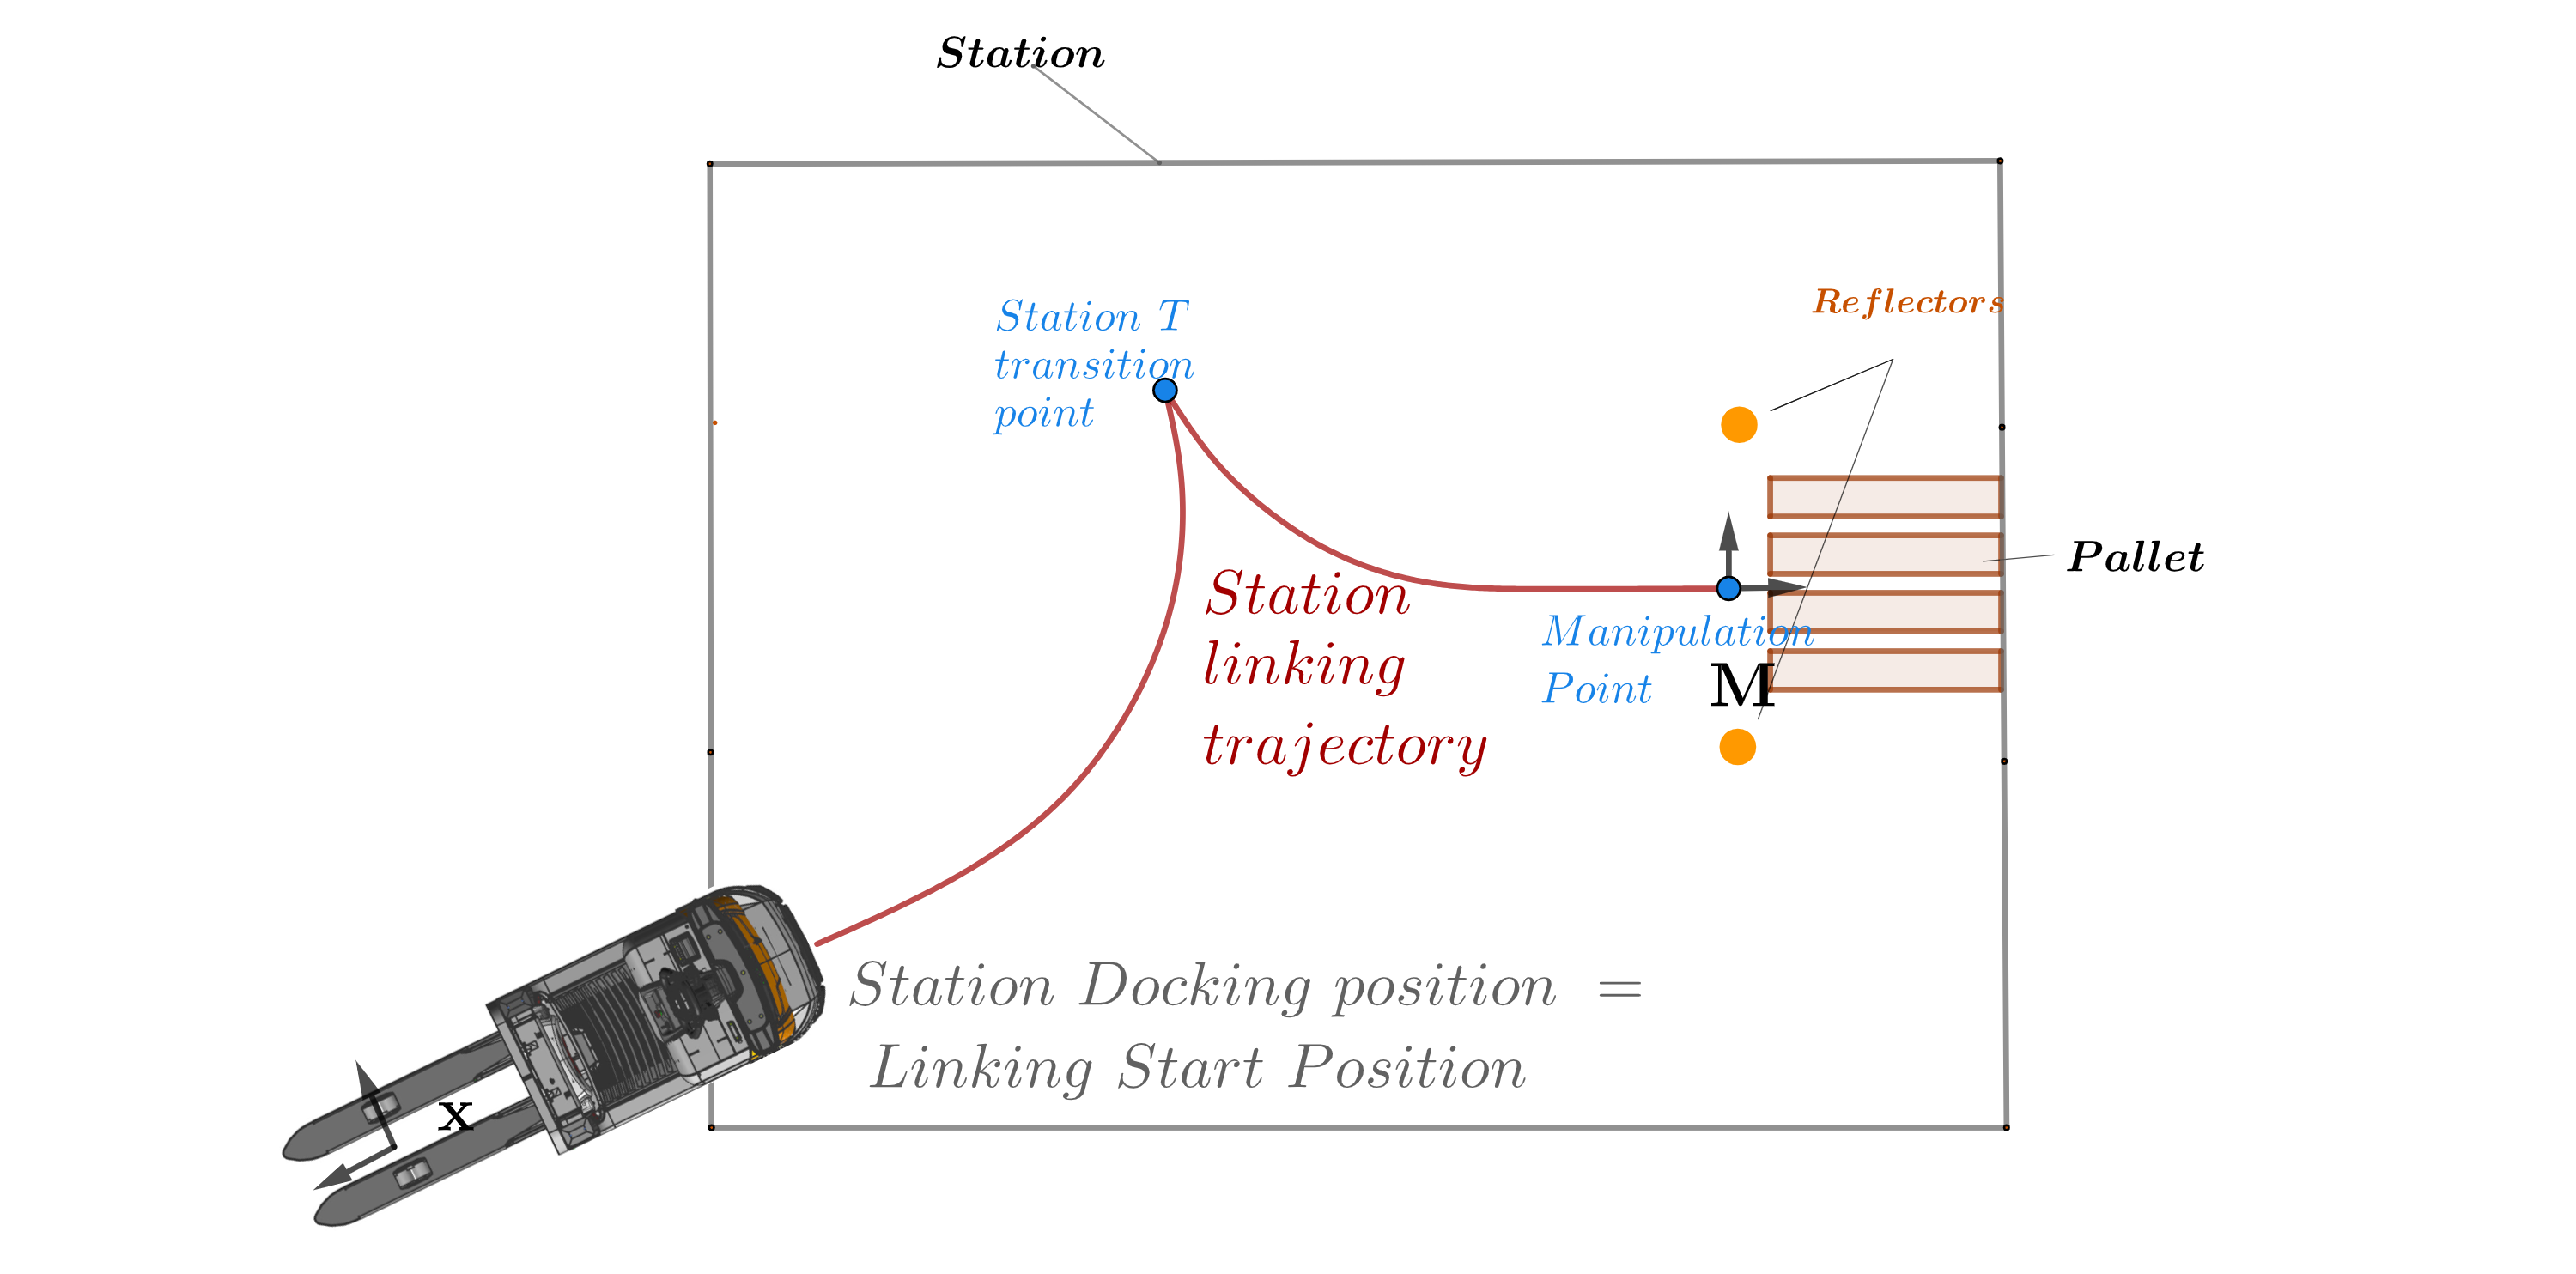
\includegraphics[width=4in]{images/Chap2/station-without-subpolygones.png}\\
    \caption{Linking the robot to goal pallet}
    \label{pattern}
    \end{center}
\end{figure}
